%Paulin VIOLETTE
%Si t'as pas bossé sur l'interface utilisateur t'y touche pas.
%Sauf si la personne dont le nom est écris en haut te dis d'y toucher.
%Deso Paulin moi j'y ai touché
\chapter{Interface Utilisateur}

\section{Présentation}

%Mettre l'image de ma super interface grave stylé
\begin{figure}[h]
  \centering
  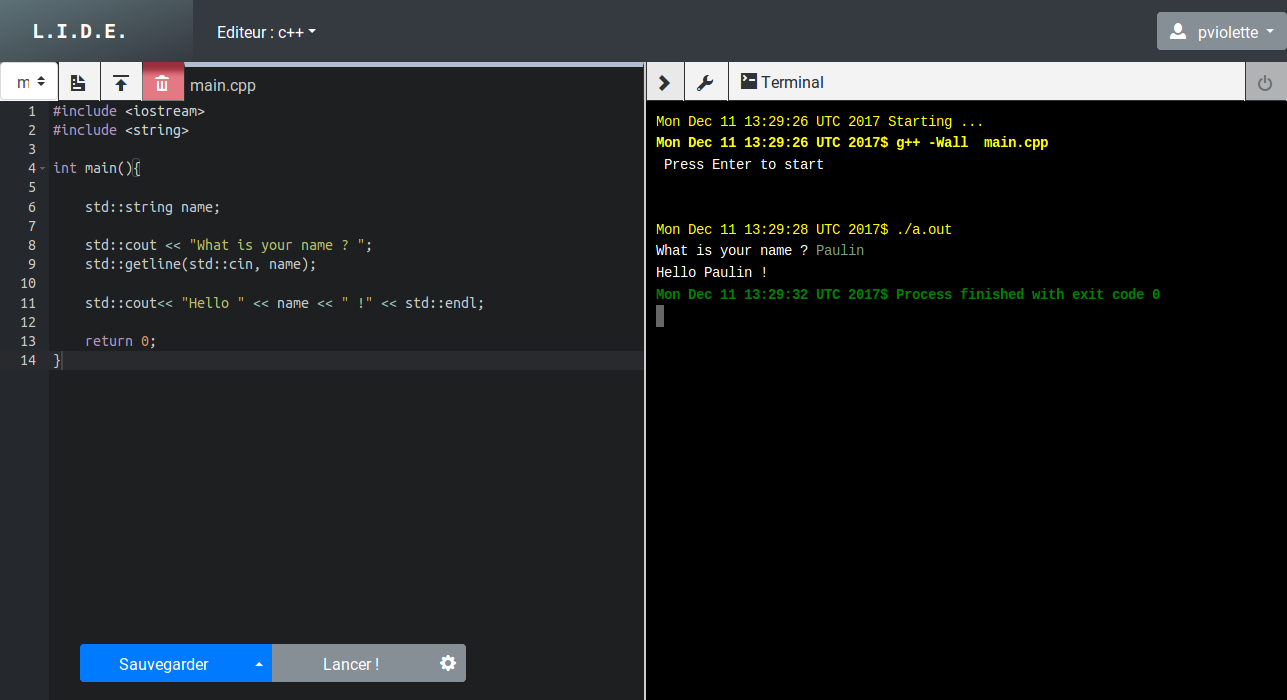
\includegraphics[width=0.8\textwidth]{./img/frontend/example1.png}
  \caption{Interface utilisateur en utilisation}
  \label{}
\end{figure}

Une fois l'utilisateur connecté, il est redirgigé vers l'interface de l'application : un éditeur de texte et une console.
L'interface est divisée en quatre parties :
\begin{itemize}
  \item La barre de navigation, contenant les liens vers les autres parties du site (gestion de compte...)
  \item La barre d'outils, qui contient des contrôles spécifiques à l'application
  \item L'editeur, implémenté par le plugin Ace
  \item La console, implémentée par le plugin jqconsole
\end{itemize}

\section{Outils utilisés}

%Blabla HTML/CSS/JS, generateur de template twig, Framework bootstrap
%Utilisation de jquery
%Editeur ace
%SweetAlert2 pour les alertes trop swag
%JQConsole vite zef parceque c'est valou qui l'a fait

\subsection{Organisation des templates TWIG}

\section{Environnement de Développement}

\subsection{Gestions des langages}
Blabla DB changement de langage

\subsection{Éditeur de texte}
Tres court parce que y'a pas grand chose à dire

\subsection{Personnalisation}

Toute personne ayant travaillé en groupe sur un projet informatique a pu remarquer que chacun à ses préférences de thème pour un éditeur : certains préfèrent un fond sombre, d'autres un fond clair, etc...
L'éditeur Ace est facilement personnalisable et dispose, par défaut, de 24 thèmes. Il était donc assez rapide d'implémenter un formulaire permettant à l'utilisateur de choisir le thème qui lui convient le mieux, lui permettant ainsi de facilement s'approprier son outil de travail.

La police est également personnalisable, permettant à chacun d'utiliser une taille de police qui lui convient.

La console ayant un style implémenter par le CSS, il fut de même aisé de créer des thèmes qui s'appliquent grâce à une classe attribuée à l'élément div contenant la console.
Pour l'instant, seul trois styles de console sont implémenter, mais il serait aisé d'en ajouter d'autres dans des versions futures.
Chaque style a une classe maîtresse \emph{.console-nom\_style}, et on redéfinit ensuite les classes \emph{jqconsole} grâce aux sélecteurs CSS. Voir le fichier \emph{console.css}.

Tous ces changements sont pour l'instant uniquement gérer en local (voir fichier \emph{options.js}).

\begin{figure}[!h]oir le fichier \emph{console.css}.
\centering
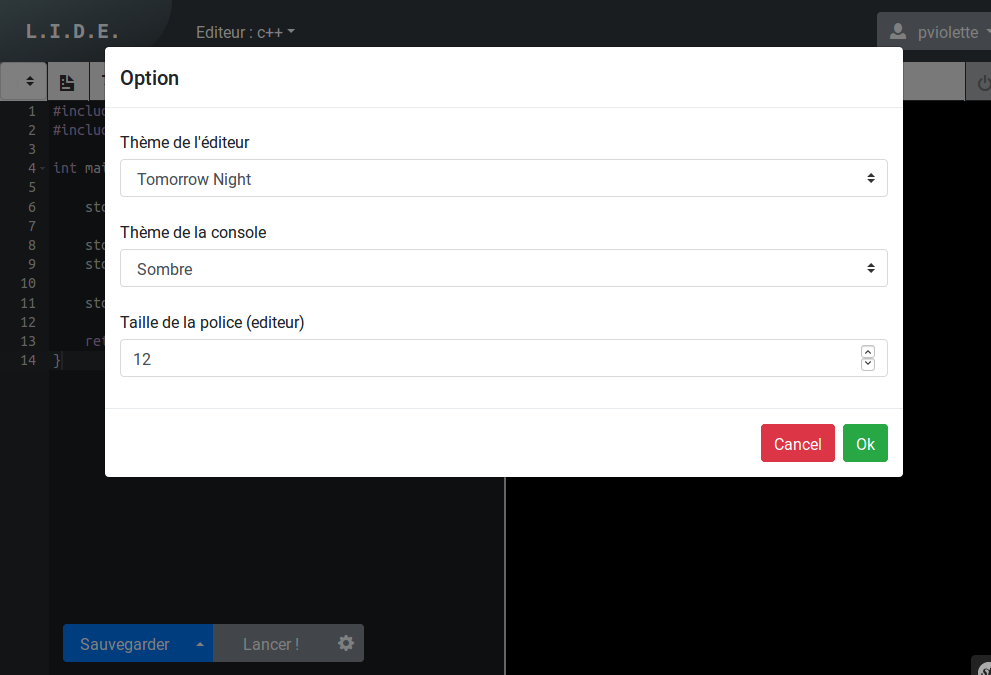
\includegraphics[width=0.8\textwidth]{./img/frontend/example_personnalisation.png}
\caption{Formulaire permettant la personnalisation de l'interface}
\end{figure}

\subsection{Gestions des fichiers}
Tel un véritable EDI, notre application permet la gestion de multiples fichiers. Cette gestion est effectuée sur le navigateur par du javascript.

Les fichiers sont enregistrés dans un prototype contenant deux champs : \emph{name}, le nom du fichier, et \emph{content} son contenu. Ces prototypes sont ensuite stockés dans la variable globale \emph{files}, un tableau de fichier. À chaque changement de fichier en cours d'édition, le contenu de l'éditeur est sauvegardé et est ensuite remplacé par le contenu du nouveau fichier à éditer.

Les fichiers peuvent être créer de deux façons : soit en important un fichier depuis son ordinateur (bouton importation), soit par création à partir de modèles définis par l'administrateur pour le langage.
On laisse également la possibilité de créer des fichiers vides (par exemple pour créer un fichier de données utilisé lors de l'exécution du programme).


\section{Compilation et exécution}

\subsection{Formulaire}


\subsection{Lancement de la compilation et de l'exécution}

Le lancement de la compilation et de l'exécution du code écrit est demandé par l'appui sur le bouton "Lancer" qui appelle une fonction JS envoyant une requête AJAX
vers la méthode ConsoleController::execAction (fichier ConsoleController.php). Cette requête contient le formulaire qui est ensuite traité : les fichiers vont être écrits dans
le système du fichier dans un dossier temporaire, le script de lancement et d'exécution correspondant au langage est récupéré dans la base de donnée et placé dans ce même répertoire.
Une commande, qui va permettre de lancer le docker, est ensuite construite. Cette commande va :
\begin{itemize}
  \item Stopper le container de l'utilisateur s'il existe.
  \item{Lancer un container basé sur l'image correspondante au langage, de nom \emph{id\_[id\_user]A}, paramétré pour être supprimé à la fin de l'exécution de la commande de lancement. Cette commande de lancement va :
  \begin{itemize}
    \item Récupérer le script de lancement sur le serveur de l'application via un wget
    \item Attribuer les droits d'exécution sur ce script
    \item Une commande sed remplaçant les caractères indésirables (dus à la base de données).
    \item Lancer le script avec les bons paramètres
  \end{itemize}}
\end{itemize}

Les paramètres du script à lancer sont :
\begin{itemize}
  \item -o 'options\_de\_compilation', pour les paramètres à passer au compilateur
  \item -f 'fichier1 fichier2...'', la liste des fichiers de l'utilisateur (récupérée par un wget)
  \item -i fichier, le nom du fichier contenant les inputs s'il est nécessaire
  \item -n, pour un mode non interactif.
  \item -a 'agr0 arg1 ...', les arguments à donner au programme
  \item -c, pour uniquement effectuer la compilation
  \item -w 'wget\_adr' l'adresse où effectuer le wget.
\end{itemize}

\subsection{Terminal}

\par La mise en place de la console proposait deux options : soit la création d'une vue ad-hoc soit l'intégration d'une vue déjà existante.

\par Notre choix s'est vite tourné vers l'intégration d'une vue déjà existante. La création d'une vue nous aurait certes donné une modularité de la console en ce qui concerne les modifications mais, la console une fois implémentée n'a pas nécessairement besoin de mofications.

\par Après étude de rentabilité, nous avons décidé d'implémenter la vue JQConsole \footnote{https://github.com/replit/jq-console} qui correspondait exactement à nos besoins. En plus d'être esthétique, son code source était placé sous licence libre et toutes les fonctions qui nous étaient nécessaires étaient déjà implémentées. L'inconvénient principal est que la modification du code source peut se montrer compliqué, celui-ci étant rédigé en CoffeeScript et étant assez compliqué.

\par Nous n'avions donc plus qu'à intégrer la vue JQConsole à notre interface et faire appel aux bonnes fonctions (notamment JQConsole.Write qui permet d'afficher du texte dans la console et JQConsole.Prompt qui permet de lire du texte) pour obtenir notre console.

\section{Problème rencontré et amélioration possible}

\subsection{Rendre l'interface Responsive}
